\subsection{Langkah Praktikum: Pewarnaan Graf dengan Backtracking}
Praktikum 7 menerapkan backtracking untuk pewarnaan graf. Graf disimpan sebagai adjacency list, lalu warna dicoba dari warna pertama sampai warna terakhir.

\begin{figure}[H]
    \centering
    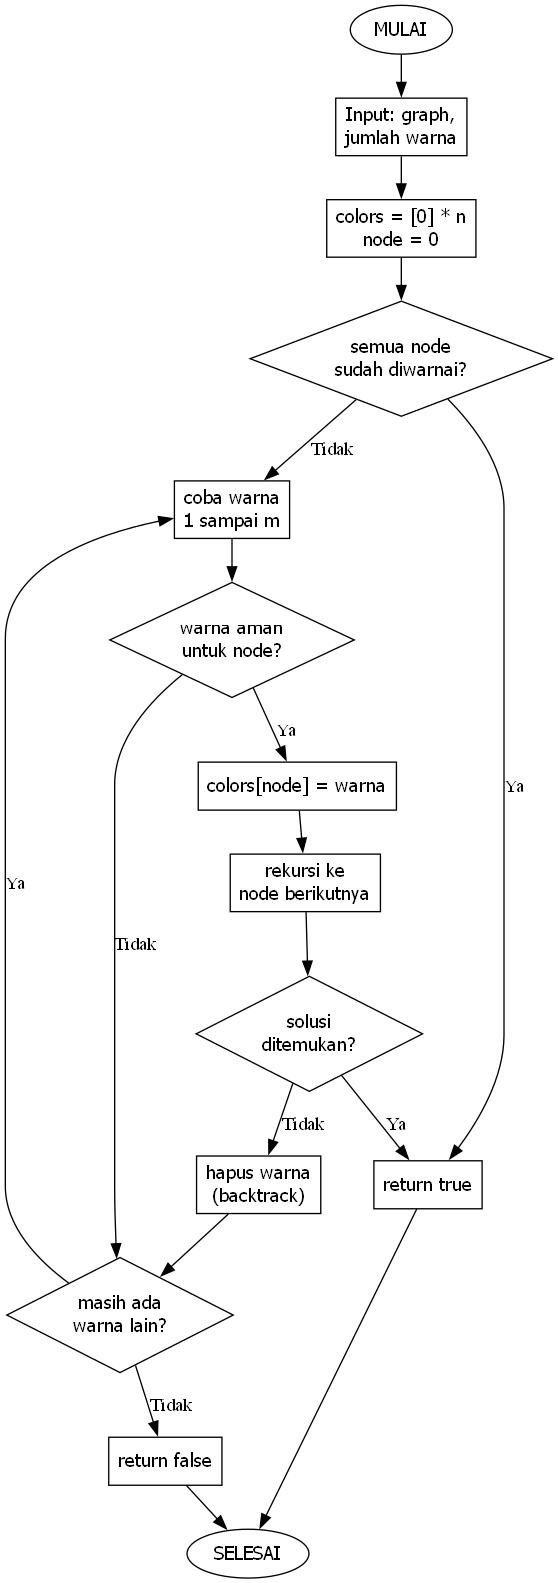
\includegraphics[width=0.52\textwidth]{figures/praktikum7/flowchart_backtracking.png}
    \caption{Flowchart Algoritma Backtracking untuk Pewarnaan Graf}
    \label{fig:praktikum7-flowchart-backtracking}
\end{figure}

\subsubsection*{Source Code Python}
Source code lengkap terdapat pada folder \texttt{src/praktikum7}. Bagian berikut hanya menampilkan inti program.

\textbf{1. Fungsi pengecekan warna dan rekursi}
\begin{lstlisting}[basicstyle=\ttfamily\scriptsize, frame=single, backgroundcolor=\color{white}, numbers=none, keywordstyle=\color{black}, commentstyle=\color{black}, stringstyle=\color{black}, breaklines=true]
def is_safe(graph, colors, node, color):
    for neighbor in graph[node]:
        if colors[neighbor] == color:
            return False
    return True


def color_graph_backtracking(graph, num_colors, node=0, colors=None):
    if colors is None:
        colors = [0] * len(graph)

    if node == len(graph):
        return True, colors

    for color in range(1, num_colors + 1):
        if is_safe(graph, colors, node, color):
            colors[node] = color

            solved, result = color_graph_backtracking(
                graph, num_colors, node + 1, colors
            )
            if solved:
                return True, result

            colors[node] = 0

    return False, colors
\end{lstlisting}

\textbf{2. Kode tester}
\begin{lstlisting}[basicstyle=\ttfamily\scriptsize, frame=single, backgroundcolor=\color{white}, numbers=none, keywordstyle=\color{black}, commentstyle=\color{black}, stringstyle=\color{black}, breaklines=true]
praktikum_edges = [
    (0, 1), (0, 2), (0, 3), (1, 2), (1, 3), (1, 4),
    (1, 5), (2, 3), (2, 5), (3, 4), (4, 5),
]

pretest_edges = [
    (3, 4), (3, 0), (4, 1), (0, 1), (0, 2), (1, 2),
]

run_case("Graf praktikum Gambar 7.4", 6, praktikum_edges, 4)
run_case("Graf pre/post test Gambar 7.5", 5, pretest_edges, 3)
\end{lstlisting}

\subsubsection*{Analisis}
\textbf{Hasil graf praktikum:}
\begin{table}[H]
    \centering
    \caption{Hasil Pewarnaan Graf Contoh Praktikum}
    \label{tab:praktikum7-hasil-praktikum}
    \begin{tabular}{ll}
    \toprule
    \textbf{Aspek} & \textbf{Hasil} \\ \midrule
    Jumlah simpul & 6 \\
    Jumlah warna & 4 \\
    Solusi kode warna & [1, 2, 3, 4, 1, 4] \\
    Solusi nama warna & [Merah, Hijau, Biru, Kuning, Merah, Kuning] \\ \bottomrule
    \end{tabular}
\end{table}

\textbf{Post Test: Pewarnaan Graf Gambar 7.5}
\begin{table}[H]
    \centering
    \caption{Validasi Hasil Program vs Manual pada Graf Gambar 7.5}
    \label{tab:praktikum7-validasi-posttest}
    \begin{tabular}{lll}
    \toprule
    \textbf{Sumber} & \textbf{Solusi Kode Warna} & \textbf{Solusi Nama Warna} \\ \midrule
    Manual Pre Test & [1, 2, 3, 2, 1] & [Merah, Hijau, Biru, Hijau, Merah] \\
    Program Python & [1, 2, 3, 2, 1] & [Merah, Hijau, Biru, Hijau, Merah] \\ \bottomrule
    \end{tabular}
\end{table}

\textbf{Kesimpulan:} Program menghasilkan pewarnaan yang valid karena setiap simpul bertetangga memiliki warna berbeda. Hasil post test sama dengan jawaban manual.
